%%%%%%%%%%%%%%%%%%%%%%%%%%%%%%%%%%%%
\miguel{For scientific research: reviewed by other peers, reproducible (data + sources, matching the article), Open Access.
One quality criteria: reproducibility. Define "reproducibility" and "repeatability". Different levels of reproducibility. Bottom level:
black box (being able to obtain the same results given the same inputs). Higher level: full access to a well-commented source code, and checking
that the pseudocode matches well the implementation. In the case of a scientific publication, checking that the implementation matches exactly
what the descriptions in the article.}

% DONE -> \miguel{Indeed,having a section in the final document where we give definitions of "quality", "software", "research software", etc. is
% quite convenient. It doesn't mean other definitions are not possible, but we need to settle clearly what we're discussing in our own context.}
% Criteria of quality (brainstorming, to complete by everybody)
% DONE -> in introduction and this section \dg{We should first define what we understand by software. We can reuse the definition in FAIR4RS.}
% DONE -> section Metadata \dg{We should look at the FAIR4RS reports for the alignment for quality dimensions. In a sense, this is what FAIR aims (at a basic level).}
% DONE -> \dg{Missing the initial table here, although we had only summaries. We should see how each of those papers defined software quality dimensions.}
% DONE -> \eli{Concerning Quality Definition, there are various software models and standards that can be referred.
% However, the most recent ones are ISO and IEEE. Existing models and standards provide a full set of software characteristics: unfortunately
% they quite often have different meaning and do not have a match with software metrics used to measure software characteristics.}
% DONE -> \miguel{Perhaps the definition of quality and the classification should appear first in the document. First this section, and then Landscaping.}
%%%%%%%%%%%%%%%%%%%%%%%%%%%%%%%%%%%%

An important notion in software engineering is \textit{quality}, understood as a series of desirable particularities that are met in \textit{good} computer programs, meaning that they are well adapted to their purpose, accurate, highly available, or any other property which makes it excellent.
Whereas this is a concept which is easy to understand, arriving at a consensus on how to properly define is a way more complex task. Indeed, the problem can be address from plenty of different perspectives, each of them giving more or less importance to some of the particularities.

It is not the goal in this report to propose any particular definitions, but to analyse how the problem has been addressed in significant works in the literature and how the characteristics can be classified as attributes.

In Section~\ref{subsect:sqchar} we shall review which are, according to the literature, the \textit{characteristics} that might be related to good software. From this list, we discuss which of the characteristics are very significant to assess the quality of software, and we shall refer to these special characteristics as \textit{attributes}, that we classify in Section~\ref{subsec:SW_quality_attributes}.

\subsection{Software Quality models: Survey}

A survey has been conducted by the subgroup and follows the methodology proposed by Kitchenham and Charters \cite{keele2007guidelines} consisting of the following steps:

\begin{enumerate}
    \item Source selection and search: We have searched in the Scopus dataset, including the top five journals in software engineering related to software \footnote{\url{https://research.com/journals-rankings/computer-science/software-programming}} and articles of the  ``International Conference on Software Engineering", one of the top venues for Software engineering. We also added documents and web resources that the Task Force subgroup considered relevants. The search included the keywords ``software quality" in the title of the target publications.
    \item Inclusion and exclusion criteria: Excluded journals not in the SE domain. Excluded articles not written in English.
    \item Selection procedure: Skim article titles and abstracts. The process was performed by 2-3 people. Final list was agreed upon by the group through discussion about the relevance of the paper and analysis if that paper contains or proposes Software Quality attributes.
    \item Review process: After following the selection procedure, we ended up with 19 articles, which have been reviewed in this survey. Some of the articles refer to the ISO/IEC 25010:2011(E)\cite{iso_25010_2011_2017} or to its precursor ISO/IEC 9126, have been grouped together.
\end{enumerate}

The journals that where considered are: "IEEE Transactions on Software Engineering", "Empirical Software Engineering", "Journal of Systems and Software", "Software \& Systems Modeling", "Information and Software Technology", "IEEE Software", "Software Quality Journal". The following query was used:

\tiny
\begin{verbatim}
    TITLE ( software  AND quality )  AND  
        ( LIMIT-TO ( EXACTSRCTITLE ,  "Software Quality Journal" )  
        OR  LIMIT-TO ( EXACTSRCTITLE ,  "Proceedings International Conference On Software Engineering" ) 
        OR  LIMIT-TO ( EXACTSRCTITLE ,  "IEEE Transactions on Software Engineering" )
        OR  LIMIT-TO ( EXACTSRCTITLE ,  "Empirical Software Engineering" ) 
        OR  LIMIT-TO ( EXACTSRCTITLE ,  "Journal of Systems and Software" ) 
        OR  LIMIT-TO ( EXACTSRCTITLE ,  "Software & Systems Modeling" ) 
        OR  LIMIT-TO ( EXACTSRCTITLE ,  "Information and Software Technology" )  
        OR  LIMIT-TO ( EXACTSRCTITLE ,  "IEEE Software" )   
        )  AND  ( LIMIT-TO ( SUBJAREA ,  "COMP" )  OR  LIMIT-TO ( SUBJAREA ,  "ENGI" ) )  
\end{verbatim}
\small

As a result, the subgroup obtained 272 results. Additional selection excluded:

\begin{itemize}
    \item Papers with no abstracts.
    \item Proceedings/workshop summary.
    \item Those which did not seem related by browsing the abstract and title.
    \item Papers that did not seem to propose quality dimensions (e.g., if they talk about practices).
\end{itemize}

There where 147 papers remaining after the abovementioned selection to which 4 more documents where added, they were not published as paper but considered relevant by the subgroup. In the end of this process, there were 19 articles remaining that were reviewed by 2-3 persons each.

% Query: \footnote{\url{https://www.scopus.com/results/results.uri?sort=plf-f&src=s&nlo=&nlr=&nls=&sid=b04451f7b887660ce99d73bfdbdc4fc8&sot=a&sdt=a&cluster=scosubjabbr%2c%22COMP%22%2ct%2c%22ENGI%22%2ct%2bscoexactsrctitle%2c%22Software+Quality+Journal%22%2ct%2c%22Proceedings+International+Conference+On+Software+Engineering%22%2ct%2c%22IEEE+Transactions+on+Software+Engineering%22%2ct%2c%22Empirical+Software+Engineering%22%2ct%2c%22Journal+of+Systems+and+Software%22%2ct%2c%22Software+%26+Systems+Modeling%22%2ct%2c%22Information+and+Software+Technology%22%2ct%2c%22IEEE+Software%22%2ct&sl=30&s=TITLE+%28+software+AND+quality+%29&cl=t&offset=201&origin=resultslist&ss=plf-f&ws=r-f&ps=r-f&cs=r-f&cc=10&txGid=cff6749bf8a084912200dbef379950d4} 
% Also, this book: https://books.google.es/books?hl=en&lr=&id=XTvpAQAAQBAJ&oi=fnd&pg=PR3&dq=software+quality&ots=fohz_-KW0d&sig=5TGlvR3sgAIkAHzs5Iup8Qijpuo#v=onepage&q=software%20quality&f=false looks nice!

\subsection{Software Quality characteristics}
\label{subsect:sqchar}

We identified a list of significant quality characteristics mainly from three sources:

\begin{itemize}
    \item The ISO/IEC 25010:2011(E) standard~\cite{iso_25010_2011_2017};
    \item The ISO/IEC/IEEE 24765:2010(E) standard~\cite{iso_central_secretary_isoiecieee_2010};
    \item The chapter \textit{Design Fundamentals} of the Microsoft Application Architecture Guide~\cite{microsoft_2010}.
\end{itemize}

The ISO/IEC/IEEE 24765:2010(E) settles a common vocabulary for systems and software engineering, in a way that it is always applicable to general applications. This standardised list provides a vast quantity of very precise definitions that avoid trivial misinterpretations, and that therefore we apply in this report.

\miguel{The ISO/IEC/IEEE 24765:2010(E) standard has been deprecated in favour of ISO/IEC/IEEE 24765:2017. Are we using anything very related to :2010, or can we use :2017?}

The ISO/IEC 25010:2011(E) is a recent (2017) norm that proposes two models for the characteristics. The first group is related to the context on which the software product is used, and contains five characteristics. The second group has eight characteristics according to characteristics of the software of computer system itself, without relying on how it is used.

The chapter Quality Attributes from Microsoft's Application Architecture Guide also helped establishing a common terminology in our definitions.

The analysis of the existing literature resulted in a significant number of characteristics which were associated to the concept of quality. All the characteristics were taken into account in our study, but some of them where filtered out since they were not useful to perform the classification in quality attributes. Indeed, some of the characteristics were pertinent at the time of the publication of the article, but after a few years they became obsolete. For example, producing a very small compiled binary is \textit{per se} an indication of quality does not make much sense these days, when in the past it could be directly related to the ability of storing the program in a very limited memory or permanent media. Other characteristics were discarded because they were very specific to an application domain, such as real-time or critical systems. They remain valid characteristics to take into account, but they are not general enough or not applicable to Research Software.

The end result was 25 significant quality characteristics from the three abovementioned sources.

\textbf{Functional suitability}: Degree to which a product or system provides functions that meet stated and implied needs when used under specified conditions.

\textbf{Availability}: Degree to which a system, product or component is operational and accessible when required for use, adapted from \cite{iso_central_secretary_isoiecieee_2010}.

\textbf{Reliability}: Degree to which a system, product or component performs specific functions under specified conditions for a specified period of time, adapted from \cite{iso_central_secretary_isoiecieee_2010}. \textbf{Notes}: Limitations in reliability are due to faults in requirements, design and implementation, or due to contextual changes.

\textbf{Time behaviour}: Degree to which the response and processing times and throughput rates of a product or system, when performing its functions, meet requirements.

\textbf{Performance}: Performance relative to the amount of resources used under stated conditions. \textbf{Notes}: Resources can include other software products, the software and hardware configuration of the system, and materials (e.g. print paper, storage media).

\textbf{Ease of use (Usability)}: Degree to which a product or system can be used by specified users to achieve specific goals with effectiveness, efficiency and satisfaction in a specified context of use. \textbf{Notes}: Adapted from ISO 9241-210. Usability can either be specified or measured as a product quality characteristic in terms of its sub-characteristics, or specified or measured directly by measures that are a subset of quality in use.

\textbf{Fault tolerance}: Degree to which a system, product or component operates as intended despite the presence of hardware or software faults, adapted from \cite{iso_central_secretary_isoiecieee_2010}.

\textbf{Security}: Degree to which a product or system protects information and data so that persons or other products or systems have the degree of data access appropriate to their types and levels of authorisation. \textbf{Notes}: As well as data stored in or by a product or system, security also applies to data in transmission. Survivability (the degree to which a product or system continues to fulfil its mission by providing essential services in a timely manner in spite of the presence of attacks) is covered by recoverability (4.2.5.4). Immunity (the degree to which a product or system is resistant to attack) is covered by integrity (4.2.6.2). Security contributes to trust (4.1.3.2).

\textbf{Maintainability}: Degree of effectiveness and efficiency with which a product or system can be modified by the intended maintainers. \textbf{Notes}: Modifications can include corrections, improvements or adaptation of the software to changes in environment, and in requirements and functional specifications. Modifications include those carried out by specialised support staff, and those carried out by business or operational staff, or end users. Maintainability includes installation of updates and upgrades. Maintainability can be interpreted as either an inherent capability of the product or system to facilitate maintenance activities, or the quality in use experienced by the maintainers for the goal of maintaining the product or system.

\textbf{Recoverability}: Degree to which, in the event of an interruption or a failure, a product or system can recover the data directly affected and re-establish the desired state of the system. \textbf{Notes}: Following a failure, a computer system will sometimes be down for a period of time, the length of which is determined by its recoverability.

\textbf{Operability / Manageability}: Degree to which a product or system has attributes that make it easy to operate and control. \textbf{Notes}: Operability corresponds to controllability, (operator) error tolerance and conformity with user expectations as defined in ISO 9241-110.

\textbf{Resource utilisation}: Degree to which the amounts and types of resources used by a product or system, when performing its functions, meet requirements. \textbf{Notes}: Human resources are included as part of efficiency (4.1.2).

\textbf{Safety}: Degree to which a product or system mitigates the potential risk to people in the intended contexts of use.

\textbf{Interoperability}: Degree to which two or more systems, products or components can exchange information and use the information that has been exchanged, adapted from \cite{iso_central_secretary_isoiecieee_2010}.

\textbf{Attractiveness}: Renamed as user interface aesthetics. Degree to which a user interface enables pleasing and satisfying interaction for the user. \textbf{Notes}: This refers to properties of the product or system that increase the pleasure and satisfaction of the user, such as the use of colour and the nature of the graphical design.

\textbf{Compatibility}: Degree to which a product, system or component can exchange information with other products, systems or components, and/or perform its required functions, while sharing the same hardware or software environment, adapted from \cite{iso_central_secretary_isoiecieee_2010}.

\textbf{Installability}: Degree of effectiveness and efficiency with which a product or system can be successfully installed and/or uninstalled in a specified environment.

\textbf{Technical accessibility}: Degree to which a product or system can be used by people with the widest range of characteristics and capabilities to achieve a specified goal in a specified context of use. \textbf{Notes}: The range of capabilities includes disabilities associated with age. Accessibility for people with disabilities can be specified or measured either as the extent to which a product or system can be used by users with specified disabilities to achieve specified goals with effectiveness, efficiency, freedom from risk and satisfaction in a specified context of use, or by the presence of product properties that support accessibility.

\textbf{Portability / Adaptability}: Degree of effectiveness and efficiency with which a system, product or component can be transferred from one hardware, software or other operational or usage environment to another, adapted from \cite{iso_central_secretary_isoiecieee_2010}. \textbf{Notes}: Portability can be interpreted as either an inherent capability of the product or system to facilitate porting activities, or the quality in use experienced for the goal of porting the product or system.

\textbf{Modifiability}: Degree to which a product or system can be effectively and efficiently modified without introducing defects or degrading existing product quality. \textbf{Notes}: Implementation includes coding, designing, documenting and verifying changes. Modularity (4.2.7.1) and analysability (4.2.7.3) can influence modifiability. Modifiability is a combination of changeability and stability.

\textbf{Reusability}: Degree to which an asset can be used in more than one system, or in building other assets.

\textbf{Scalability}: 1.) Scalability is the ability of a system to either handle increases in load without impact on the performance of the system, or the ability to be readily enlarged \cite{microsoft_2010} $OR$ 2.) Scalability is the capability of algorithms, protocols, and applications to efficiently handle a growing amount of work or the demand of increasing its performance (according to some metrics) by adding resources to the system in which the software is running. Resources can be added to the single nodes (vertical scalability) and to the system as a whole (horizontal scalability) \cite{bondi_2000}.

\textbf{Supportability}: 1.) Supportability is the ability of the system to provide information helpful for identifying and resolving issues when it fails to work correctly \cite{microsoft_2010} $OR$ 2.) Existence of a helpdesk or issue tracking, bug reporting, enhancements and general support \cite{orviz_fernandez_eosc-synergy_2020}.

\textbf{Testability}: Degree of effectiveness and efficiency with which test criteria can be established for a system, product or component and tests can be performed to determine whether those criteria have been met, adapted from \cite{iso_central_secretary_isoiecieee_2010}.

\textbf{Confidentiality}: Degree to which a product or system ensures that data are accessible only to those authorised to have access.

\subsection{Software Quality attributes}
\label{subsec:SW_quality_attributes}

The result of the survey was a total of 241 Quality Attributes. All attributes were gathered in a table and some were aggregated into a single attribute when they were from different sources but with the same (or very similar) definition or meaning.

The subgroup ended up with 132 Quality Attributes after aggregation and the list is shown in Appendix~\ref{appendix_qa}. All paper sources have been referenced. The metrics and attributes where subdivided into six categories and for each metric or attribute, a new codename was created by the subgroup in order to have a coherent naming convention throughout the document:

\begin{itemize}
    \item Source Code Metrics (\textbf{EOSC-SCMet}): 20 metrics.
    \item Time metrics (\textbf{EOSC-TMet}): 11 metrics. Metrics related to time or periods time.
    \item Qualitative Attributes (\textbf{EOSC-Qual}): 30 attributes. Qualitative attributes are obtained in general through surveys to or some manual analysis: SW developers, SW administrators, users. (Are not fit, or not possible to automatize).
    \item DevOps - SW release and management Attributes (\textbf{EOSC-SWRelMan}): 34 attributes. Based largely in DevOps, most can be automated for verification.
    \item DevOps - Testing Attributes (\textbf{EOSC-SWTest}): 25 attributes. Based in DevOps, most can be automatically verified.
    \item Service Operability Attributes (\textbf{EOSC-SrvOps}): 12 attributes. Scientific services or platforms in operation.
\end{itemize}

Figure \ref{fig:sqattr} depicts what is shown in Appendix~\ref{appendix_qa} for each metric or attribute.

\begin{figure}[h]
    \centering
    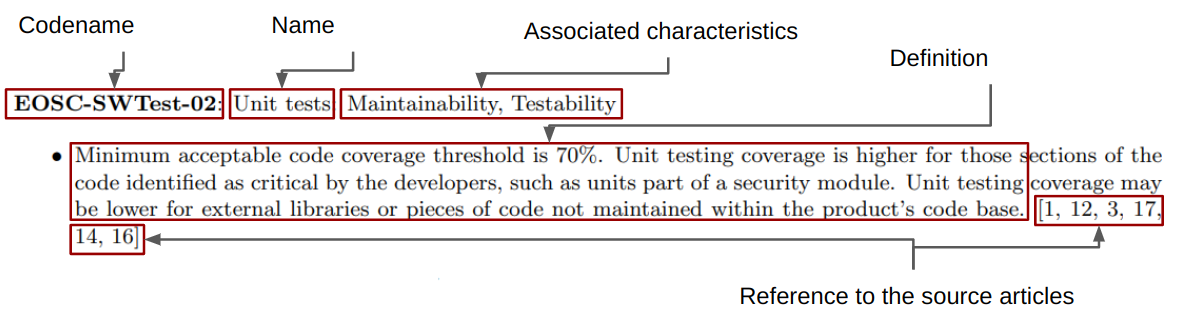
\includegraphics[width=0.99\linewidth]{imgs/qa.png}
    \caption{Software Quality Attribute.}
    \label{fig:sqattr}
\end{figure}

For each attribute it's shown:

\begin{itemize}
    \item Attribute codename: naming convention created by the subgroup.
    \item Attribute name: from the references.
    \item Attribute characteristics: one or more from subsection \ref{subsect:sqchar}.
    \item Attribute definition: from the reference(s), can be an aggregation from more than one reference.
    \item Attribute paper references.
    \item Attribute RS level: from the user stories in subsection \ref{subsec:user_stories}.
\end{itemize}
